\section{}
A propped cantilever beam AB is supported at one end by a spring of constant stiffness $k$ and subjected to a
uniform load of intensity $p$, as shown in Fig. \ref{fig:Q1ProblemDiagram}. Use the unit-load method to determine the
deflection of the beam at its free end B.

\begin{figure}[h]
    \centering
    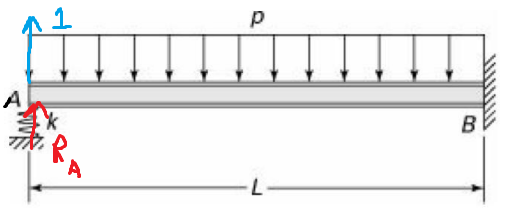
\includegraphics[width=0.5\linewidth]{Questions/Figures/Q1ProblemDiagram.png}
    \caption{Propped cantilever beam AB}
    \label{fig:Q1ProblemDiagram}
\end{figure}

First, the moment from A to B is found:
\begin{equation*}
    M = \frac{-px^2}{2} 
\end{equation*}

Apply a virtual unit load at A. The moment equation is:
\begin{equation*}
    m = (1)x
\end{equation*}

The virtual work equation is:
\begin{align*}
    \delta_{A} &= \int_{0}^{L} \frac{Mm}{EI} dx \\
    &= \frac{1}{EI} \int_{0}^{L} \left(\frac{-px^2}{2}\right)(1x) dx \\
    &= \frac{-pL^4}{8EI}
\end{align*}

By Hooke's Law, the reaction force is $R_A = -k\delta_A$. Therefore,
\begin{equation*}
    \boxed{R_A = \frac{kpL^4}{8EI}}
\end{equation*}